%%%%%%%%%%%%  Generated using docx2latex.com  %%%%%%%%%%%%%%

%%%%%%%%%%%%  v2.0.0-beta  %%%%%%%%%%%%%%

\documentclass[10pt]{article}

\usepackage{amsmath}
\usepackage{latexsym}
\usepackage{amsfonts}
\usepackage[normalem]{ulem}
\usepackage{array}
\usepackage{amssymb}
\usepackage{graphicx}



\usepackage{subfig}
\usepackage{wrapfig}
\usepackage{wasysym}
\usepackage{enumitem}
\usepackage{adjustbox}
\usepackage{ragged2e}
\usepackage[svgnames,table]{xcolor}
\usepackage{tikz}
\usepackage{longtable}
\usepackage{changepage}
\usepackage{setspace}
\usepackage{hhline}
\usepackage{multicol}
\usepackage{tabto}
\usepackage{float}
\usepackage{multirow}
\usepackage{makecell}
\usepackage{fancyhdr}
\usepackage[toc,page]{appendix}
\usepackage[hidelinks]{hyperref}
\usetikzlibrary{shapes.symbols,shapes.geometric,shadows,arrows.meta}
\tikzset{>={Latex[width=1.5mm,length=2mm]}}
\usepackage{flowchart}\usepackage[paperheight=11.69in,paperwidth=8.27in,left=1.0in,right=1.0in,top=1.0in,bottom=1.0in,headheight=1in]{geometry}
\usepackage[utf8]{inputenc}
\usepackage[T1]{fontenc}

\TabPositions{0.5in,1.0in,1.5in,2.0in,2.5in,3.0in,3.5in,4.0in,4.5in,5.0in,5.5in,6.0in,}

\urlstyle{same}


 %%%%%%%%%%%%  Set Depths for Sections  %%%%%%%%%%%%%%

% 1) Section
% 1.1) SubSection
% 1.1.1) SubSubSection
% 1.1.1.1) Paragraph
% 1.1.1.1.1) Subparagraph


\setcounter{tocdepth}{5}
\setcounter{secnumdepth}{5}


 %%%%%%%%%%%%  Set Depths for Nested Lists created by \begin{enumerate}  %%%%%%%%%%%%%%


\setlistdepth{9}


\renewlist{itemize}{itemize}{9}
		\setlist[itemize]{label=$\cdot$}
		\setlist[itemize,1]{label=--}
		\setlist[itemize,2]{label=-}
		\setlist[itemize,3]{label=$\ast$}
		\setlist[itemize,4]{label=$\dagger$}
		\setlist[itemize,5]{label=$\triangleright$}
		\setlist[itemize,6]{label=$\bigstar$}
		\setlist[itemize,7]{label=$\blacklozenge$}
		\setlist[itemize,8]{label=$\prime$}



 %%%%%%%%%%%%  Header here  %%%%%%%%%%%%%%




\renewcommand{\headrulewidth}{0pt}
\setlength{\topsep}{0pt}\setlength{\parindent}{1em}

 %%%%%%%%%%%%  This sets linespacing (verticle gap between Lines) Default=1 %%%%%%%%%%%%%%


\renewcommand{\arraystretch}{1.3}

\renewcommand{\labelitemi}{--}

\let\tempone\itemize
\let\temptwo\enditemize
\renewenvironment{itemize}{\tempone\setlength\itemsep{-0.5pt}}{\temptwo}

\let\tempeone\enumerate
\let\tempetwo\endenumerate
\renewenvironment{enumerate}{\tempeone\setlength\itemsep{-0.5pt}\setlength{\partopsep}{-0.5pt}\setlength{\parsep}{-0.5pt}\setlength{\topsep}{-0.5pt}}{\tempetwo}


\title{Data model for citations in dictionaries}
\author{Katrien Depuydt, Jesse de Does}
\date{}


%%%%%%%%%%%%%%%%%%%% Document code starts here %%%%%%%%%%%%%%%%%%%%


\begin{document}

\maketitle
\par



\begin{abstract}
    

 In a dictionary article, lexicographers cite other resources to substantiate their analysis. These citations can be found everywhere in the dictionary, eg. in the etymological section of a dictionary article, in the definition of an entry etc.

 A special form of citations are those that function as examples to give evidence, elucidate meaning or illustrate features (spelling variation, syntax, collocation, register (etc)).  These citations are a representative selection of occurrences of the headword from either a corpus of texts or a corpus of snippets from texts. These citations, i.e. attestations, usually occur in the form of a quote with bibliographical information. In some cases, only a few context words are given, not the actual attested word form, in other cases, only the bibliographical reference is given.
 
 
 Attestations are attributed examples in a dictionary. There are usage examples that are not attributed. They are either invented or based on corpus material, but adapted/simplified by the lexicographer. We 
 will focus on attestations.

\end{abstract}
\section{Introduction}
\addcontentsline{toc}{section}{Introduction}
Lexicographers use examples  to support their analysis of the headword. The examples can either be authentic (exact quotations), adapted (modified versions of authentic examples) or invented examples (\cite{Svensen}, p. 283-285). Authentic examples are attributed quotations (citations), which not only elucidate meaning and illustrate features of the headword (spelling, syntax, collocation, register etc.), but also function as attestations and are used provide evidence of the existence of a headword (\cite{AtkinsRundell}, p. 453-458). We therefore call these examples ``attestations''. Adapted examples, (cf\.~a.o.~\cite{ColloCaid}, p. 251) or invented examples, which often occur in learner's dictionaries and bilingual dictionaries (\cite{Kernerman}), will not be discussed here.  \par


\section{Citations and attestations in scholarly dictionaries}
\addcontentsline{toc}{section}{Citations and attestations in scholarly dictionaries}

In ``scholarly dictionaries'' (OED, ANW, the major historical dictionaries of Dutch\footnote{\url{http://gtb.ivdnt.org}}, TLFI, Lewis and Short, Liddell and Scott, Böhtlingk and Roth, Hanyu Da Cidian, ...), the main role of citations and quotations is 
\begin{enumerate}
    \item To illustrate usage
    \item To provide evidence for the lexicographical interpretation of a word sense (``attestation'')
\end{enumerate}

As stated by Hawke, \cite{Hawke} p. 176, ``The quotation evidence is the bedrock of any historical dictionary. The relationship between the definitions of each sense in a historical dictionary and the quotations that accompany it is particulary close. In the compilation of a historical dictionary (at least in modern times) the quotation evidence provides a sample of the empirical data on which the definitions have been based''

Thus, it is important to be explicit about the nature of the evidence provided. The dictionary should provide information on the reliability of attestations; this information should also be represented in the knowledge base. 

\subsection{Reliability of attestations}

\addcontentsline{toc}{subsection}{Reliability of attestations}


 An attestation is as good as the corpus text or quotation the attestation is taken from. The analysis of the lexicographer as such can also be subject to discussion.\par

\subsubsection*{Uncertain reading or reconstruction}
\addcontentsline{toc}{subsubsection}{Uncertain reading or reconstruction}


For historical dictionaries, the source material consists of text editions of historical documents. The further we go back in time, the more challenging it is to find enough material. Sometimes, sources have come down to us in one manuscript or a few manuscript fragments, with parts that are hard to read, or only partially legible (think of a hole in a manuscript). Or the word in question is misspelled.\par


The impact of this on the lexicographer’s work is, that some of the $``$evidence$"$  in a quotation is in fact a reconstruction\footnote{Another matter, which will briefly discussed in section \ref{ssec:witness}, is to be explicit about what the attestation actually provides evidence for in terms of the temporal and regional distribution of the phenomenon attested. For this purpose, the metadata provided with the quotations should accurately represent the nature of the source text from which the quotation has been taken.}.\par



\paragraph*{Some examples}

 In the Dictionary of Old Dutch, the entry with the Dutch adverb \textit{fora }has related entries, one of which refers to a placename \textit{foraskōta}. The editor suggests a correction of a spelling in the third quotation.\par




%%%%%%%%%%%%%%%%%%%% Figure/Image No: 1 starts here %%%%%%%%%%%%%%%%%%%%
\begin{figure}[H]
	\begin{Center}
		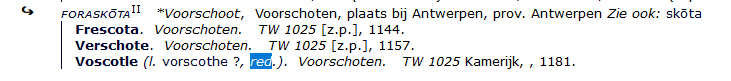
\includegraphics[width=6.27in,height=0.69in]{./image18.png}
	\end{Center}
	\caption{example: Spelling correction proposed by editor}
\end{figure}
%%%%%%%%%%%%%%%%%%%% Figure/Image No: 1 Ends here %%%%%%%%%%%%%%%%%%%%



 Another example is from the Dictionary of Early Middle Dutch, where the fourth attestation has an occurrence of the verb \textit{staen }(to stand), which is partly a reconstruction: s[tut].\par



%%%%%%%%%%%%%%%%%%%% Figure/Image No: 2 starts here %%%%%%%%%%%%%%%%%%%%
\begin{figure}[H]
	\begin{Center}
		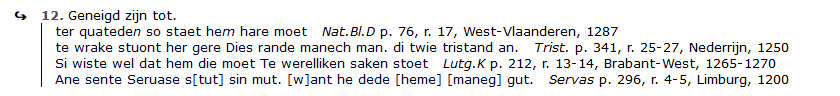
\includegraphics[width=6.27in,height=0.72in]{./image15.png}
	\end{Center}
	\caption{example: reconstructed reading}
\end{figure}
%%%%%%%%%%%%%%%%%%%% Figure/Image No: 2 Ends here %%%%%%%%%%%%%%%%%%%%


These corrections or reconstructions are recognizable. According to the lexicographer, they are valid examples of the meaning of the entry. However, as representative of the spelling, they are not so reliable.\par



\subsubsection*{Uncertain interpretation}
\addcontentsline{toc}{subsubsection}{Uncertain interpretation}



Sometimes, there may not be any doubt about the reading of a quoted passage of a source text, but the lexicographer is uncertain about his/her interpretation. In this example, the lexicographer gives a potential $``$misschien ook (maybe also)$"$  other interpretation of an attestation.

\bigskip

\begin{figure}[H]
\begin{minipage}{14cm}
{
\small
\textit{In onderstaande aanh.~is behalve een acc.pl.~}\textbf{\textit{misschien ook}}  een interpretatie als znw.v. met als bet.~'bank(instelling)' mogelijk (vgl. MNW IV, 746-749).


 Oec\ mach\ die greue van vyanen lombarde houden binnen sinen sonderlinghen lande,   \href{http://gtb.ivdnt.org/iWDB/search?actie=article&wdb=VMNWBRONNEN&id=1646}{\textit{\uline{Corp.I}}} p. 2470, r. 20-21, Grimbergen, Brabant-West, 1298
}
\end{minipage}
\caption{example: doubt about interpretation}
\end{figure}


\subsection{Citations as evidence: different types}
\addcontentsline{toc}{subsection}{Citations as evidence: different types}


 There are several ways in which a citation as evidence can occur (list might not be exhaustive).\par



\begin{enumerate}
	\item  A bibliographical reference is given

	\item The attested wordform is quoted in context + the bibliographical reference is given

	\item Some context words are given, accompanied by a bibliographical reference.
\end{enumerate}



\paragraph*{Example of a and b}

 In the Dictionary of the Dutch language, the quotation section begins with a listing of the dictionaries that describe the entry in the same meaning, followed by a group of quotations + bibliographical information with attestations (bold) of the entry in this quotation\par



%%%%%%%%%%%%%%%%%%%% Figure/Image No: 3 starts here %%%%%%%%%%%%%%%%%%%%
\begin{figure}[H]
	\begin{Center}
		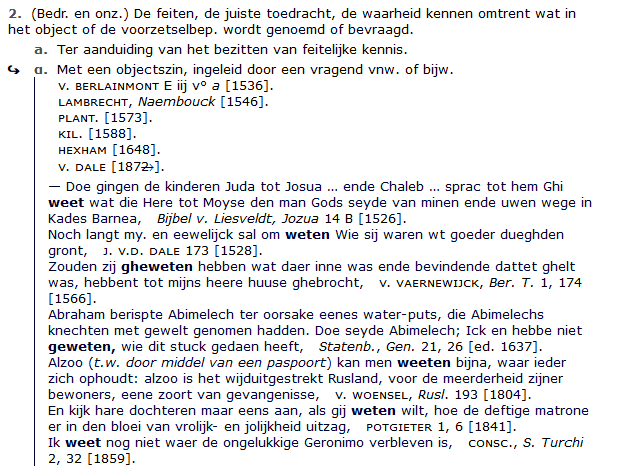
\includegraphics[width=5.14in,height=3.93in]{./image19.png}
	\end{Center}
\end{figure}
%%%%%%%%%%%%%%%%%%%% Figure/Image No: 3 Ends here %%%%%%%%%%%%%%%%%%%%


\paragraph*{An example of a and c}

 In the Liddell Scott Jones lexicon, bibliographical references are given, or a description of the type of context the entry word was found in.

%%%%%%%%%%%%%%%%%%%% Figure/Image No: 4 starts here %%%%%%%%%%%%%%%%%%%%
\begin{figure}[H]
\advance\leftskip 0.12in		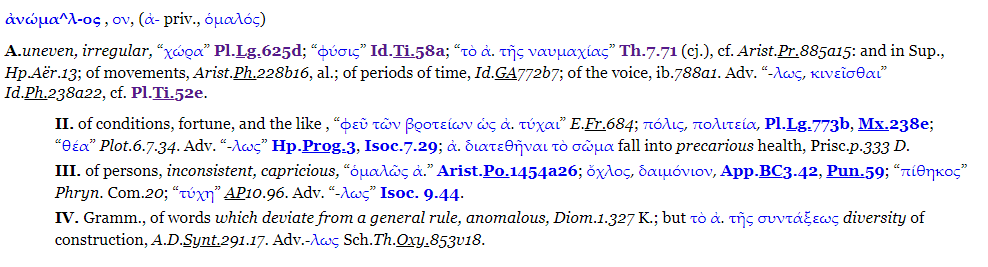
\includegraphics[width=6.27in,height=1.69in]{./image14.png}
\end{figure}
%%%%%%%%%%%%%%%%%%%% Figure/Image No: 4 Ends here %%%%%%%%%%%%%%%%%%%%

\par

\subsection{Linked data modeling of lexical citations}
\addcontentsline{toc}{subsection}{Linked data modeling of lexical citations}


The concept of attestations is discussed in two recent publications. One is the publication on the model for the DiaMaNT lexicon (\cite{DEPUYDT18.25}). The most recent publication is the one by Khan and Boschetti \cite{KhanBoschetti}.  This article on lexical attestations prompted us to re-evaluate the proposal for attestations in Depuydt en Does 2018. We will discuss briefly the model by \cite{KhanBoschetti} and will then come up with an alternative proposal.



\subsubsection*{Khan and Boschetti}
\addcontentsline{toc}{subsubsection}{1. Khan and Boschetti}




%%%%%%%%%%%%%%%%%%%% Figure/Image No: 5 starts here %%%%%%%%%%%%%%%%%%%%
\begin{figure}[H]
	\begin{Center}
		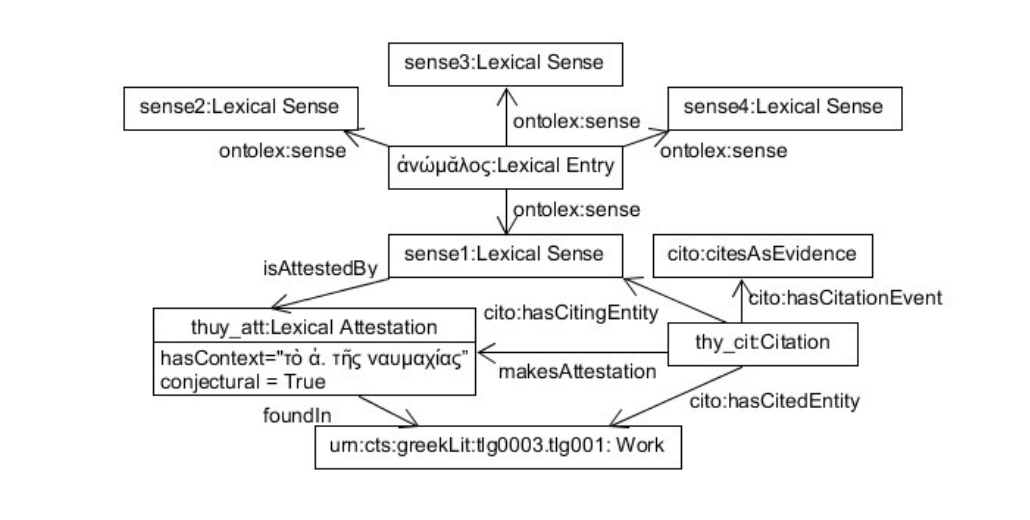
\includegraphics[width=6.27in,height=3.6in]{./image10.png}
	\end{Center}
	\caption{Example modeling from \cite{KhanBoschetti}}
\end{figure}
%%%%%%%%%%%%%%%%%%%% Figure/Image No: 5 Ends here %%%%%%%%%%%%%%%%%%%%

 Khan and Boschetti’s \textit{lemonBib} model for lexiographical citations tackles some issues important for historical lexicography and proposes solutions based on the FRBR, Cito and Fabio ontologies\cite{PeroniShotton}

\begin{itemize}
\item Distinction between citation in general and a citation which provides evidence for a certain lexical object (\textit{Attestation}) (Word sense, word form, $ \ldots $ .)

\item	Enabling the marking of text readings as conjectural

\item The distinction between a $``$work$"$  and its $``$Manifestation$"$  in the form of a publication.
\end{itemize}

In our view, the resulting model\footnote{\url{http://lari-datasets.ilc.cnr.it/lemonBib}} has some drawbacks.

\begin{itemize}
\item In the K$\&$B model, the presence of context entails attestation (the \textit{hasContext }data property has domain \textit{Attestation}). The model does not take into account citations with context snippets that are \textit{not} attestations, eg. citations in a section on etymology, where an authority is quoted to back up or contradict an analysis.

	\item There appears to be an unneccessary amount of relation-reifying objects in the model. 


\end{itemize}

In the simplest application of the Cito model, $``$cites$"$  is essentially a relation between two resources representing publications, without any intermediate reifying objects. Ported to the lexical domain, this would consist of a relation between a lexical sense and a work containing an occurrence of this sense. \\
Since we want to attach some characterizations to the citation, some degree of reification is necessary, for which purpose Cito proposes the Citation class. K$\&$ B proceed by modeling Citation and Attestation as different resources with a relation \textit{attestationCitation/makesAttestation }between them. We do not see why one could not declare Attestation as a subclass of Citation and characterize them, for instance, by (e.g.)

\begin{itemize}
	\item {\fontsize{10pt}{12.0pt}\selectfont Attestation is a subclass of Citation\par}\par

	\item {\fontsize{10pt}{12.0pt}\selectfont Attestation is a subclass of (hasCitationCharacterization cito:citesAsEvidence)\par}
\end{itemize}








\subsubsection*{Alternative proposal}
\addcontentsline{toc}{subsubsection}{2. Alternative proposal}


 In Depuydt $\&$  De Does 2018, we proposed a model for attestations in which all dictionary quotations with context that illustrate word senses are also attestations (which reflects the reality of our dictionaries). The $``$Attestation$"$  object proposed there included a pointer to the location of the headword in the quotation. We considered this useful because\par

\begin{itemize}
	\item  It allows attestations of  word forms (so users can related specific word forms to document metadata, e.g. period or location)

	\item  It allows the immediate use of dictionary quotations for computational applications like WSD
\end{itemize}\par

 After reading Khan and Boschetti’s paper we realized it was important to take into account that the presence of context and the fact that the quotation provides evidence for the word sense are distinct dimensions.



 In fact, a model should be able to deal with the following situations:

{

\begin{enumerate}
	\item {\fontsize{10pt}{12.0pt}\selectfont attestation, no doubt about reading or interpretation}

\begin{enumerate}
	\item {\fontsize{10pt}{12.0pt}\selectfont only mentioning the source\par}

	\item {\fontsize{10pt}{12.0pt}\selectfont source with a context [with or without keyword in it]\par}\par

	\item {\fontsize{10pt}{12.0pt}\selectfont acknowledgment of the source with context and pointer \par}\par


\end{enumerate}
	\item {\fontsize{10pt}{12.0pt}\selectfont attestation, uncertain reading\par}

\begin{enumerate}
	\item {\fontsize{10pt}{12.0pt}\selectfont only source indication, is attestation, uncertain reading\par}\par

	\item {\fontsize{10pt}{12.0pt}\selectfont source with context [whether or not with keyword in it], is attestation, uncertain reading\par}\par

	\item {\fontsize{10pt}{12.0pt}\selectfont source with context and poi\setlength{\topsep}{-3\parskip}nter, is attestation, uncertain reading\par}\par


\end{enumerate}
	\item {\fontsize{10pt}{12.0pt}\selectfont attestation, uncertain interpretation\par}\par

\begin{enumerate}
	\item {\fontsize{10pt}{12.0pt}\selectfont only source indication, is attestation, uncertain interpretation\par}\par

	\item {\fontsize{10pt}{12.0pt}\selectfont source with context [with or without keyword in it], is attestation, uncertain interpretation\par}\par

	\item {\fontsize{10pt}{12.0pt}\selectfont source indication with context and pointer, attestation,uncertain interpretation\par}\par


\end{enumerate}
	\item {\fontsize{10pt}{12.0pt}\selectfont not an attestation, different type of quotation\par}\par

\begin{enumerate}
	\item {\fontsize{10pt}{12.0pt}\selectfont only source indication, is not an attestation\par}\par

	\item {\fontsize{10pt}{12.0pt}\selectfont source mention with context [with or without keyword in it], is not an attestation\par}\par

	\item {\fontsize{10pt}{12.0pt}\selectfont [theoretically] source with context and pointer, is not an attestation\par}
\end{enumerate}
\end{enumerate}
}



\bigskip
\begin{minipage}{\textwidth}

So there are at least five dimensions:\par


\begin{enumerate}
	\item Attestation (Citation provides evidence for the word sense) $ \leftrightarrow $   other type of citation

	\item  Certainty of the reading of the source text (is the word really there?)

	\item Certainty of the interpretation (is this really an instance of the relevant word sense?)

	\item  Is a context snippet given?

    \item Is the occurrence (or multiple occurrences) of the headword in the context/snippet explicitly marked?
\end{enumerate}
\end{minipage}
\bigskip





 
 \begin{minipage}{\textwidth}
  The  simple model of figure \ref{fig:attmodel} (for readability, written in a loose description logic augmented with cartesian product) tries to provide the necessary degrees of freedom.
 \begin{itemize}
     \item 
 There always is a $``$Citation$"$  object for any type of citation. it is always linked to the lexical sense (or other $``$lexical phenomena$"$) with the $``$citation$"$  object property. The type of citation (cites as evidence, agrees with, etc, cf the CITO ontology\footnotemark{}) can be reflected in the value of cito:hasCitationCharacterization property and by subclassing Citation. \par

\item  (Un)certainty of source text reading and/or lexicographic interpretation can be modeled by two distinct boolean data properties associated with the Citation object. \par

 \item Presence of context is simply reflected by a non-empty value for the snippet data property.\par

 \item The $``$locus$"$  object can optionally be used to mark the place in the snippet in which the headword occurs (this is useful for computational applications use of dictionary quotations in e.g.).\par
 \end{itemize}
\end{minipage}
\footnotetext{\  types of citation from https://sparontologies.github.io/cito/current/cito.html:  agrees withop, citationop, cites as authorityop, cites as data sourceop, cites as evidenceop, cites as metadata documentop, cites as potential solutionop, cites as recommended readingop, cites as relatedop, cites as source documentop, cites for informationop, compilesop, confirmsop, contains assertion fromop, correctsop, creditsop, critiquesop, deridesop, describesop, disagrees withop, discussesop, disputesop, documentsop, extendsop, includes excerpt fromop, includes quotation fromop, links toop, obtains background fromop, obtains support fromop, parodiesop, plagiarizesop, qualifiesop, refutesop, replies toop, retractsop, reviewsop, ridiculesop, speculates onop, supportsop, updatesop, uses conclusions fromop, uses data fromop, uses method inop }

\begin{figure}


{\fontsize{9pt}{10.8pt}\selectfont 
\uline{Classes}

lexcit:Citation $\sqsubseteq$  cito:Citation
\ \ \textit{(a lexcit Citation is also a cito:Citation)}

lexcit:Attestation  $\sqsubseteq$  lexcit:Citation%}\par%}\par

 lexcit:Attestation $\sqsubseteq$  $ \exists $  cito:hasCitationCharacterization . cito:citesAsEvidence 

\ \ \textit{(an Attestation has citation characterization citesAsEvidence)}

lexcit:Locus\  $\sqsubseteq$  ($ \exists $  nif.beginIndex.$\top$) $\sqcap$  ($ \exists $  nif.endIndex.$\top$) $\sqcap$  ($ \exists $  lexcit.locusIn.($ \exists $  lexcit:quotation.$\top$)))

 \ \ \ \ \ \ \ \ \ \ \  \textit{(a Locus has a begin and end index and points to something which has a quotation)}

 (ontolex:Form $\sqcup$  ontolex:LexicalSense) $\sqsubseteq$  lexcit:LexicalPhenomenon

\par



\uline{Data properties}

 lexcit:quotation $\sqsubseteq$  lexcit:Citation $ \times $  xs:String \textit{(domain\ is  Citation, range is string)}

 lexcit:readingCertain $\sqsubseteq$  lexcit:Citation $ \times $  xs:Boolean%}\par}\par

 lexcit:interpretationCertain $\sqsubseteq$  lexcit:Citation $ \times $  xs:Boolean


 nif:beginIndex $\sqsubseteq$  lexcit:Locus $ \times $  xs:Integer

nif:endIndex $\sqsubseteq$  lexcit:Locus $ \times $  xs:Integer



\uline{Object properties}

 lexcit:citation $\sqsubseteq$  lexcit:LexicalPhenomenon $ \times $  lexcit:Citation

lexcit:citation $\sqsubseteq$   cito:hasCitingEntity\textbf{\textsuperscript{-}} \textit{(citation is subset of the converse of cito hasCitingEntity)}

lexcit:attestation $\sqsubseteq$  lexcit:citation

lexcit:attestation $\sqsubseteq$  lexcit:LexicalPhenomenon $ \times $  lexcit:Attestation

lexcit:locus\ \ $\sqsubseteq$   lexcit:LexicalPhenomenon $ \times $  lexcit:Locus

lexcit:locusIn\  $\sqsubseteq$  lexcit:Locus $ \times $  ($ \exists $  lexcit:quotation.$\top$)


\caption{Simple data model for quotations}
\label{fig:attmodel}
\end{figure}
}

 The examples (figure \ref{fig:ex2}), illustrate an attestation of a word sense, and an example of an attestation of both a word form and a sense.\par

\begin{rdf}[width=3cm,prefix=voorbeeld1]:aap a diamant:Beast .
:aap diamant:eats diamant:Nuts .
:Nuts diamant:kindof diamant:Food .
\end{rdf}

%%%%%%%%%%%%%%%%%%%% Table No: 1 starts here %%%%%%%%%%%%%%%%%%%%

%\begin{figure}[H]

% 			\centering

%		\includegraphics[width=\textwidth]{./example_1.pdf}
%\caption{Attestation of a sense}
%\label{fig:ex1}
% \end{figure}
 
 \begin{figure}
 \begin{tabular}{cc}
     	\includegraphics[width=\textheight, angle=90]{./example_1.pdf}  &  
     	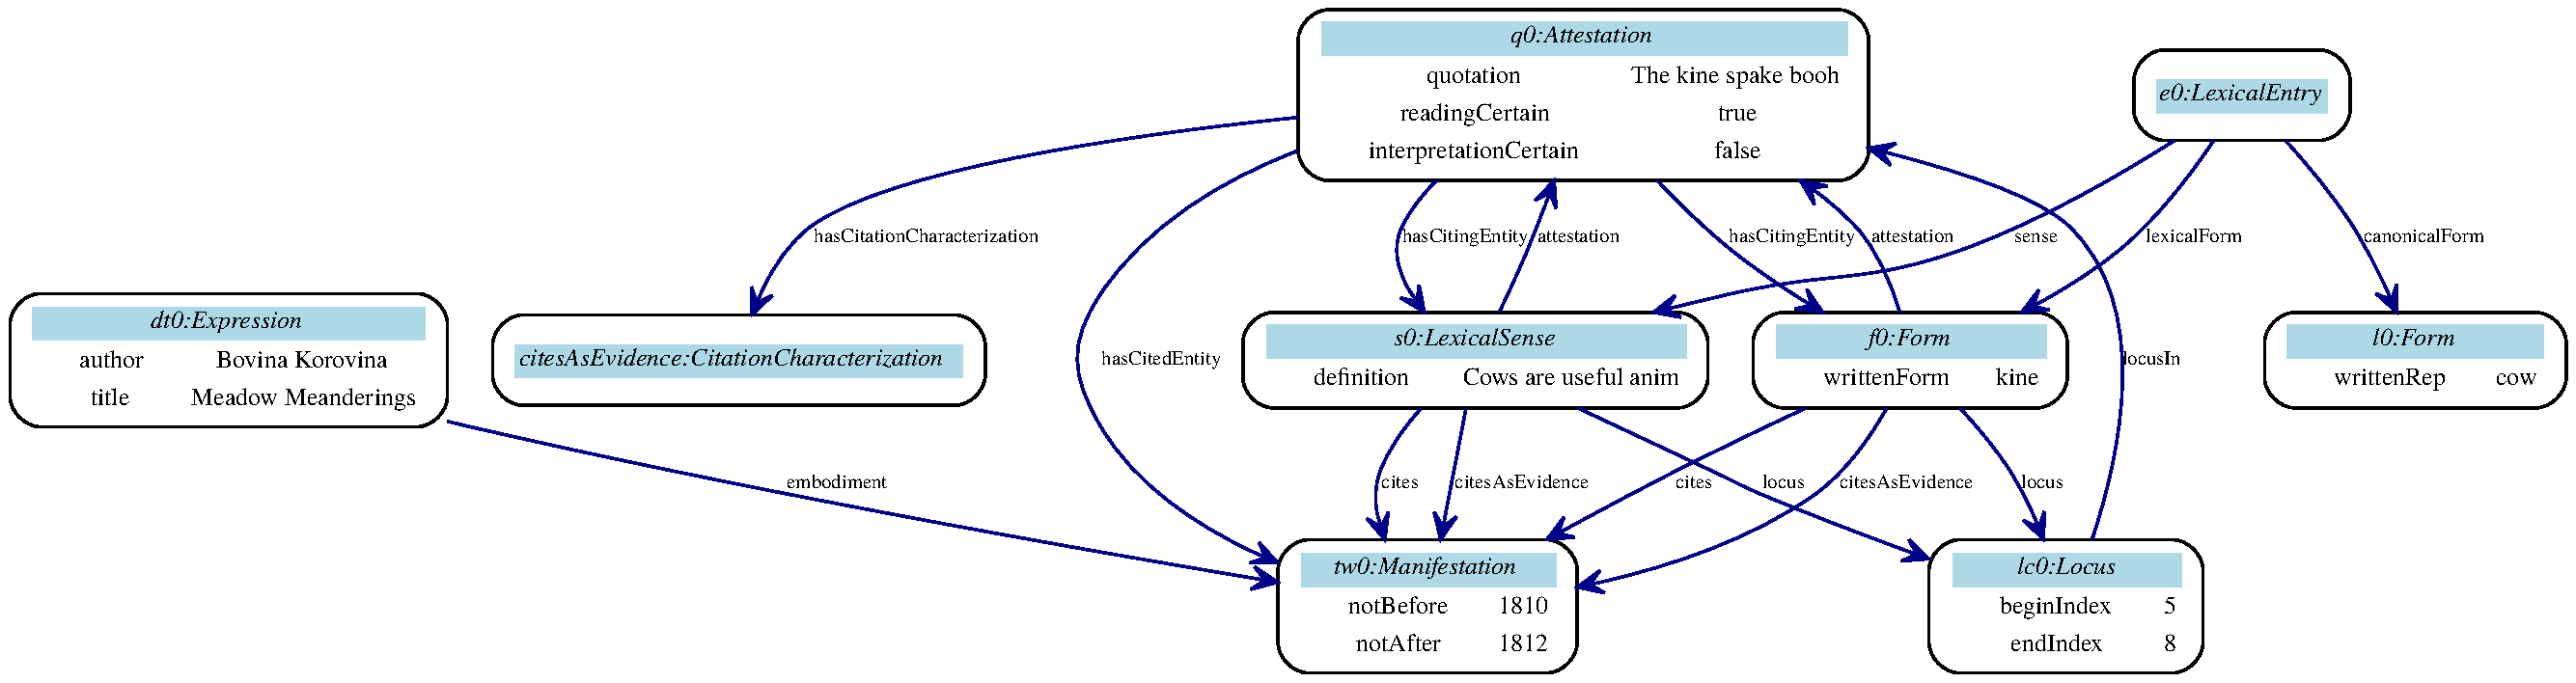
\includegraphics[width=\textheight, angle=90]{./example_2.pdf}
 \end{tabular}

\caption{Attestation of a sense (left); attestation of a sense \textit{and} a form (right) }
\label{fig:ex2}
 \end{figure}


%%%%%%%%%%%%%%%%%%%% Table No: 1 ends here %%%%%%%%%%%%%%%%%%%%





%\subsubsection*{Usage examples}
%\addcontentsline{toc}{subsubsection}{3. Usage examples}


%We have not discussed usage examples invented by lexicographers. They could simply be treated as a subclass of lexcit:Citation. Usage examples in dictionaries should have metadata just like the regular quotations: they are representative of the language of the lexicographer at a certain point in time, etc.

\subsection{Document metadata }
\label{ssec:witness}
\addcontentsline{toc}{subsection}{Document metadata }

When dealing with historical text, it is important to distinguish:


\begin{itemize}
\item The $``$text$"$ as conceived by the author(s)

\item The $``$text witness$"$  (the manuscript in which the text has come down to us)

\item The edition which gives a representation of the text witness.
\end{itemize}


 Each of these has its own metadata. For scholarly dictionaries, the text witness is important, because it determines the $``$date$"$  and the regional characteristics of the language. It is not uncommon for e.g. medieval texts that the manuscript that contains the text is dated much later than the time the text was written, and may be representative of the dialect of the copyist rather than the native dialect of the author. The language in these cases is never exactly the same, therefore the date witness is the most important. As manuscripts are usually quoted from text editions, bibliographical information of the edition the text is quoted from, is important provenance information.

To model these aspects, (as pointed out by K$\&$B), the FRBR/Fabio distinction between Works, Expressions, Manifestations and Items indeed provides us with the necessary vocabulary.
 
 We do not need the nonlinguistic ``frbr:Work'' , since there are no non-linguistic data to attest in dictionaries. So the (possibly unavailable) text as conceived by the author (or translator) corresponds to ``frbr:Expression'' and each text witness can be  considered a Manifestation.  
 
 However, both ontologies provide no means to say that the expression of the text is manifested in a manuscript which is in its turn manifested in a text edition.\par

 A further typical characteristic of dictionaries is, that the bibliographical information accompanying a quotation, is a short reference (author, title and data witness). The full bibliographical description of the resource is given separately.\par


\subsubsection*{Minimal metadata information}
\addcontentsline{toc}{subsubsection}{Minimal metadata information}


Arriving at a proposal for a common standard for attestation metadata which includes all aspects touched upon in the previous subsection is not feasible in the time frame for this document. We propose the following simple minimal model, which includes author/title/date metadata but no proposal for localization yet.


\bigskip


{\fontsize{9pt}{10.8pt}\selectfont 
\uline{Classes}

lexcit:Document\  $\sqsubseteq$  frbr:Expression

lexcit:Witness $\sqsubseteq$  frbr:Manifestation




 \uline{Data properties}

dc:title\  $\sqsubseteq$  lexcit:Document $ \times $  xs:String

dc:creator\  $\sqsubseteq$  lexcit:Document $ \times $  xs:String

lexcit:notAfter $\sqsubseteq$  lexcit:Witness $ \times $  xs:dateTime

lexcit:notAfter $\sqsubseteq$  lexcit:Witness $ \times $  xs:dateTime





\uline{Object properties}

frbr:embodiment\   $\sqsubseteq$  frbr:Expression $ \times $  frbr:Manifestation
}


\par



\bibliographystyle{acm}
\bibliography{lexcit}

 %Anas Fahad Khan $\&$  Federico Boschetti, $``$Towards a representation of citations in linked data lexical resources.$"$  In: Iztok Kosem et al., eds, \textit{Proceedings of the XVIII EURALEX International Congress: Lexicography in Global Contexts}, pages 137–147, Ljubljana, Slovenia, jul 2018. Ljubljana University Press, Faculty of Arts.\par



 %Depuydt,\ K., $\&$  de Does, J.  $``$The Diachronic Semantic Lexicon of Dutch as Linked Open Data.$"$  In I. Kernerman $\&$  S. Krek, \textit{Proceedings of the LREC 2018 Workshop $``$Globalex 2018 – Lexicography $\&$  WordNets$"$ } (pp. 23-28). Miyazaki, 2018.\par





\newpage
\section*{Appendix: Other comments on Khan and Boschetti }
\subsection*{Discussion of examples}
\addcontentsline{toc}{section}{Appendix: some remarks on the contents of Khan and Boschetti}



\subsubsection*{Provando e riprovando}



 On p.~142, it is claimed that \textit{provando e riprovando} is quoted twice. \par


\begin{figure}[H]
 \textbf{\textcolor[HTML]{3E3F3E}{riprovare$^1$ }}\textcolor[HTML]{3E3F3E}{ v. tr. [comp. di \textit{ri}- e \textit{provare}] (\textit{io ripròvo}, ecc.). – 1. \uline{Provare di nuovo, nei suoi varî sign}.: \textit{perché il vestito stia perfettamente}, \textit{sarà meglio riprovarlo}; \textit{se ci riprova}, \textit{avrà a che fare con me}; \textbf{\textit{provando e riprovando}}\textit{ quella dolcezza la quale essa prima all’altre solea biasimare}(Boccaccio); \textit{gli ho provato e riprovato la verità delle mie affermazioni}, \textit{ma non ha voluto credermi}; \uline{per il motto \textbf{\textit{provando e riprovando}}, v. provare, n. 2}. Con uso intr. (aus. \textit{avere}) o intr. pron., fare un nuovo tentativo: \textit{riprovò} (o \textit{si riprovò}) \textit{ad alzarsi e a camminare}, \textit{ma si sentì così debole che dovette quasi subito tornare a letto}. 2. ant. Saggiare monete.}\par

 \caption{Example of $``$negative attestation$"$, \textcolor[HTML]{3E3F3E}{\href{http://www.treccani.it/vocabolario/riprovare1/}{\uline{http://www.treccani.it/vocabolario/riprovare1/}}}}

\end{figure}

 Is\ \ the second mentioning (bold and underlined)  really a quotation? There is no reference to Dante here, just to the phraseme $``$provando e riprovando$"$. It might as well be considered a cross-reference to the other dictionary entry.\par



\subsubsection*{Conjectural attestation}
 On p.~143,  a Quotation of Thucydides and Aristoteles is discussed. \par







%%%%%%%%%%%%%%%%%%%% Figure/Image No: 6 starts here %%%%%%%%%%%%%%%%%%%%

\begin{figure}[H]
\advance\leftskip 0.12in		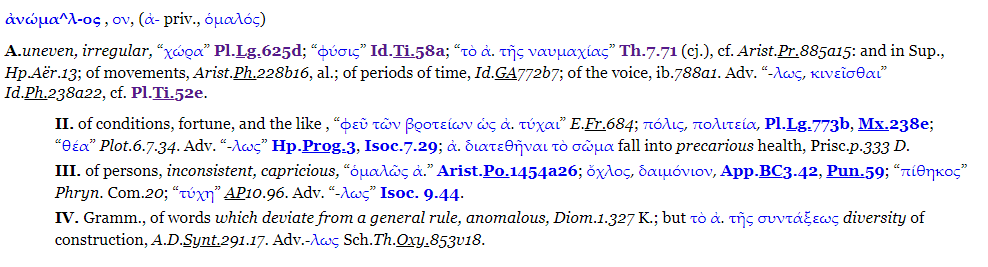
\includegraphics[width=6.27in,height=1.69in]{./image13.png}
\end{figure}


%%%%%%%%%%%%%%%%%%%% Figure/Image No: 6 Ends here %%%%%%%%%%%%%%%%%%%%

\par

 For\ the first meaning of the word, the occurrence of the entry (in this particular meaning)  in Th. is a conjecture\par



%%%%%%%%%%%%%%%%%%%% Figure/Image No: 7 starts here %%%%%%%%%%%%%%%%%%%%

\begin{figure}[H]
	\begin{Center}
		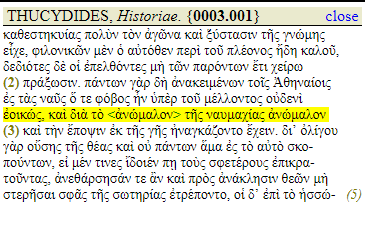
\includegraphics[width=3.8in,height=2.36in]{./image16.png}
	\end{Center}
\end{figure}


%%%%%%%%%%%%%%%%%%%% Figure/Image No: 7 Ends here %%%%%%%%%%%%%%%%%%%%

\par

 The lexicographer has added examples with a similar construction (genitive) - here one of the additional examples.\par



%%%%%%%%%%%%%%%%%%%% Figure/Image No: 8 starts here %%%%%%%%%%%%%%%%%%%%

\begin{figure}[H]
	\begin{Center}
		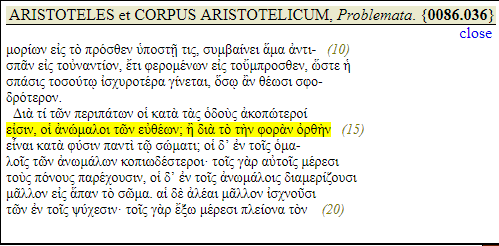
\includegraphics[width=5.2in,height=2.56in]{./image11.png}
	\end{Center}
\end{figure}


%%%%%%%%%%%%%%%%%%%% Figure/Image No: 8 Ends here %%%%%%%%%%%%%%%%%%%%

\par



 Both citations have to be treated as attestations. The Thucydides example however, is based on a reconstruction.

\newpage
\subsection*{Relation with the TEI encoding}
\addcontentsline{toc}{section}{Appendix: relation with the TEI encoding:}
 Traditional (scholarly) dictionaries use XML encoding in either an in-house format or in a standard like TEI. It is important to see the encoding as a help, and not to make it leading.\par

 Take e.g. the encoding in TEI XML of the Liddell Scott Jones lexicon. The citations without quoted text (bibl only) for instance lack the tag cit.\par



\begin{adjustwidth}{0.71in}{0.0in}
 (...)\par

\end{adjustwidth}

\begin{adjustwidth}{0.71in}{0.0in}
 <sense id="n10947.0" n="A" level="1" opt="n">\par

\end{adjustwidth}

\begin{adjustwidth}{0.85in}{0.0in}
 <tr opt="n">uneven, irregular,</tr>\par

\end{adjustwidth}

\begin{adjustwidth}{0.85in}{0.0in}
 <cit>\par

\end{adjustwidth}

\begin{adjustwidth}{0.99in}{0.0in}
 <quote lang="greek">$ \chi $ ώ$ \rho $ $ \alpha $ </quote>\par

\end{adjustwidth}

\begin{adjustwidth}{0.99in}{0.0in}
 <bibl n="Perseus:abo:tlg,0059,034:625d" default="NO" valid="yes">\par

\end{adjustwidth}

\begin{adjustwidth}{1.12in}{0.0in}
 <author>Pl.</author>\par

\end{adjustwidth}

\begin{adjustwidth}{1.12in}{0.0in}
 <title>Lg.</title>\par

\end{adjustwidth}

\begin{adjustwidth}{1.12in}{0.0in}
 <biblScope>625d</biblScope>\par

\end{adjustwidth}

\begin{adjustwidth}{0.99in}{0.0in}
 </bibl>\par

\end{adjustwidth}

\begin{adjustwidth}{0.85in}{0.0in}
 </cit>\par

\end{adjustwidth}

\begin{adjustwidth}{0.85in}{0.0in}
 ;\par

\end{adjustwidth}

\begin{adjustwidth}{0.85in}{0.0in}
 <cit>\par

\end{adjustwidth}

\begin{adjustwidth}{0.99in}{0.0in}
 <quote lang="greek">$ \varphi $ ύ$ \sigma $ $ \iota $ $ \varsigma $ </quote>\par

\end{adjustwidth}

\begin{adjustwidth}{0.99in}{0.0in}
 <bibl n="Perseus:abo:tlg,0059,031:58a" default="NO" valid="yes">\par

\end{adjustwidth}

\begin{adjustwidth}{1.12in}{0.0in}
 <author>Id.</author>\par

\end{adjustwidth}

\begin{adjustwidth}{1.12in}{0.0in}
 <title>Ti.</title>\par

\end{adjustwidth}

\begin{adjustwidth}{1.12in}{0.0in}
 <biblScope>58a</biblScope>\par

\end{adjustwidth}

\begin{adjustwidth}{0.99in}{0.0in}
 </bibl>\par

\end{adjustwidth}

\begin{adjustwidth}{0.85in}{0.0in}
 </cit>\par

\end{adjustwidth}

\begin{adjustwidth}{0.85in}{0.0in}
 ;\par

\end{adjustwidth}

\begin{adjustwidth}{0.85in}{0.0in}
 <cit>\par

\end{adjustwidth}

\begin{adjustwidth}{0.99in}{0.0in}
 <quote lang="greek">$ \tau$ ὸ ἀ. $ \tau$ ῆ$ \varsigma $  $ \nu $ $ \alpha $ $ \upsilon $ $ \mu $ $ \alpha $ $ \chi $ ί$ \alpha $ $ \varsigma $ </quote>\par

\end{adjustwidth}

\begin{adjustwidth}{0.99in}{0.0in}
 <bibl n="Perseus:abo:tlg,0003,001:7:71" default="NO" valid="yes">\par

\end{adjustwidth}

\begin{adjustwidth}{1.12in}{0.0in}
 <author>Th.</author>\par

\end{adjustwidth}

\begin{adjustwidth}{1.12in}{0.0in}
 <biblScope>7.71</biblScope>\par

\end{adjustwidth}

\begin{adjustwidth}{0.99in}{0.0in}
 </bibl>\par

\end{adjustwidth}

\begin{adjustwidth}{0.85in}{0.0in}
 </cit>\par

\end{adjustwidth}

\begin{adjustwidth}{0.85in}{0.0in}
 (cj.), cf.\par

\end{adjustwidth}

\begin{adjustwidth}{0.85in}{0.0in}
 \colorbox{Yellow}{<bibl n="Perseus:abo:tlg,0086,036:885a:15" default="NO">}\par

\end{adjustwidth}

\begin{adjustwidth}{0.99in}{0.0in}
 \colorbox{Yellow}{<author>Arist.</author>}\par

\end{adjustwidth}

\begin{adjustwidth}{0.99in}{0.0in}
 \colorbox{Yellow}{<title>Pr.</title>}\par

\end{adjustwidth}

\begin{adjustwidth}{0.99in}{0.0in}
 \colorbox{Yellow}{<biblScope>885a15</biblScope>}\par

\end{adjustwidth}

\begin{adjustwidth}{0.85in}{0.0in}
 \colorbox{Yellow}{</bibl>}\par

\end{adjustwidth}























\setlength{\parskip}{15.0pt}

\printbibliography
\end{document}

